\section*{Problem 1: Interpolation of Simple Function}


\begin{itemize}
\item
If using Chebychev polynomials with equidistant nodes, the solution for some large n is out of expectation since the matrix of basis function is close to 0 and it cause the inverse matrix unreasonable large. So if we compare the residual by comparing the solution when n increase from 5 to 15 with the function itself, we can see the pattern as follows.
\begin{figure}[htbp]
\centering
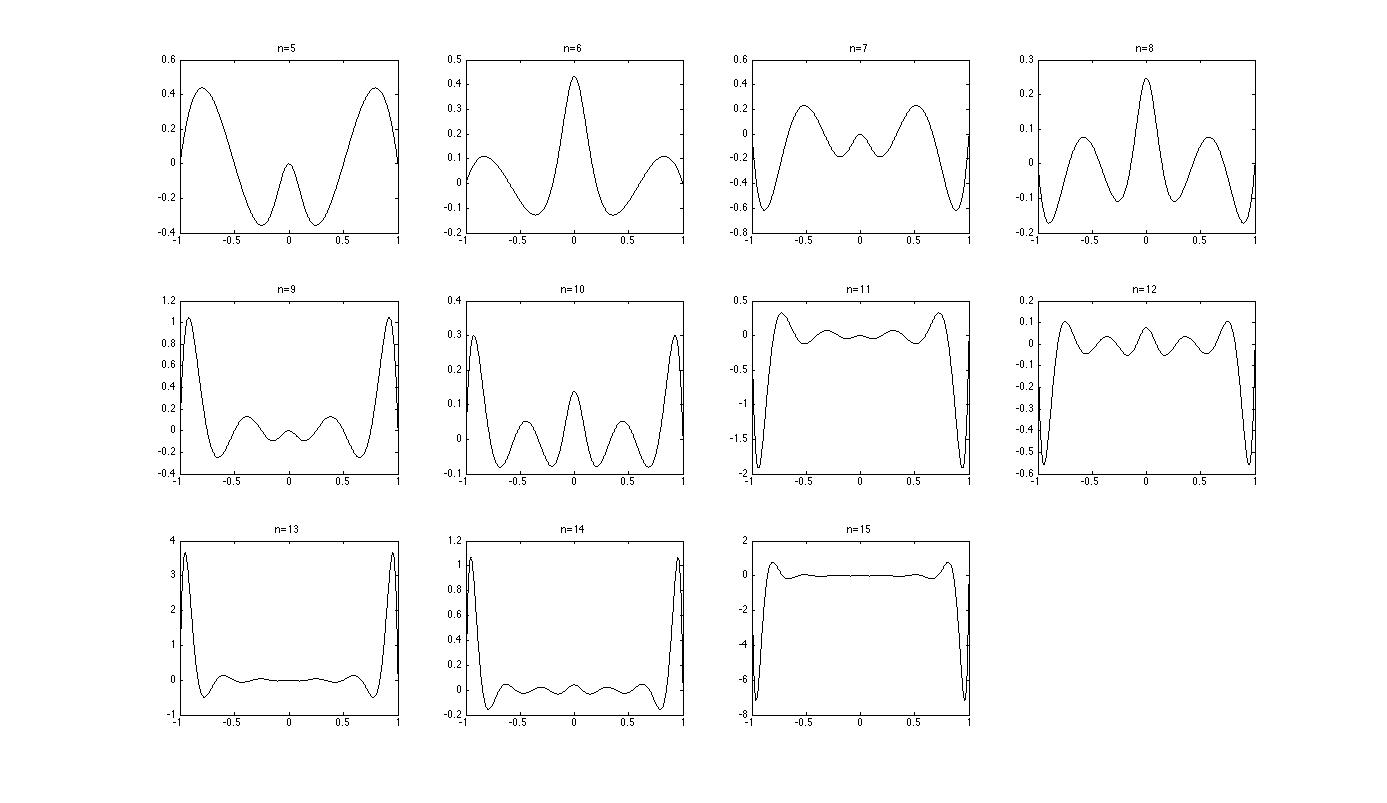
\includegraphics[width=\linewidth]{Figure/Q1_equinode.jpg}
\end{figure}
When $n$ increases, the residual converge to zero except the boundaries. It means the approximate function is more close to the exact function (except the boundaries) when the nodes increase.
\item


if using Chebychev nodes, the figure looks as follows. When $n$ increase, one significant feature contrast with former one is that the residual at boundaries are small, actually smaller than the points in the middle. Also, the residual are more close to 0 when $n$ increase, which indicates the approximate function is more close to the exact one evenly (including the boundaries).
\begin{figure}[htbp]
\centering
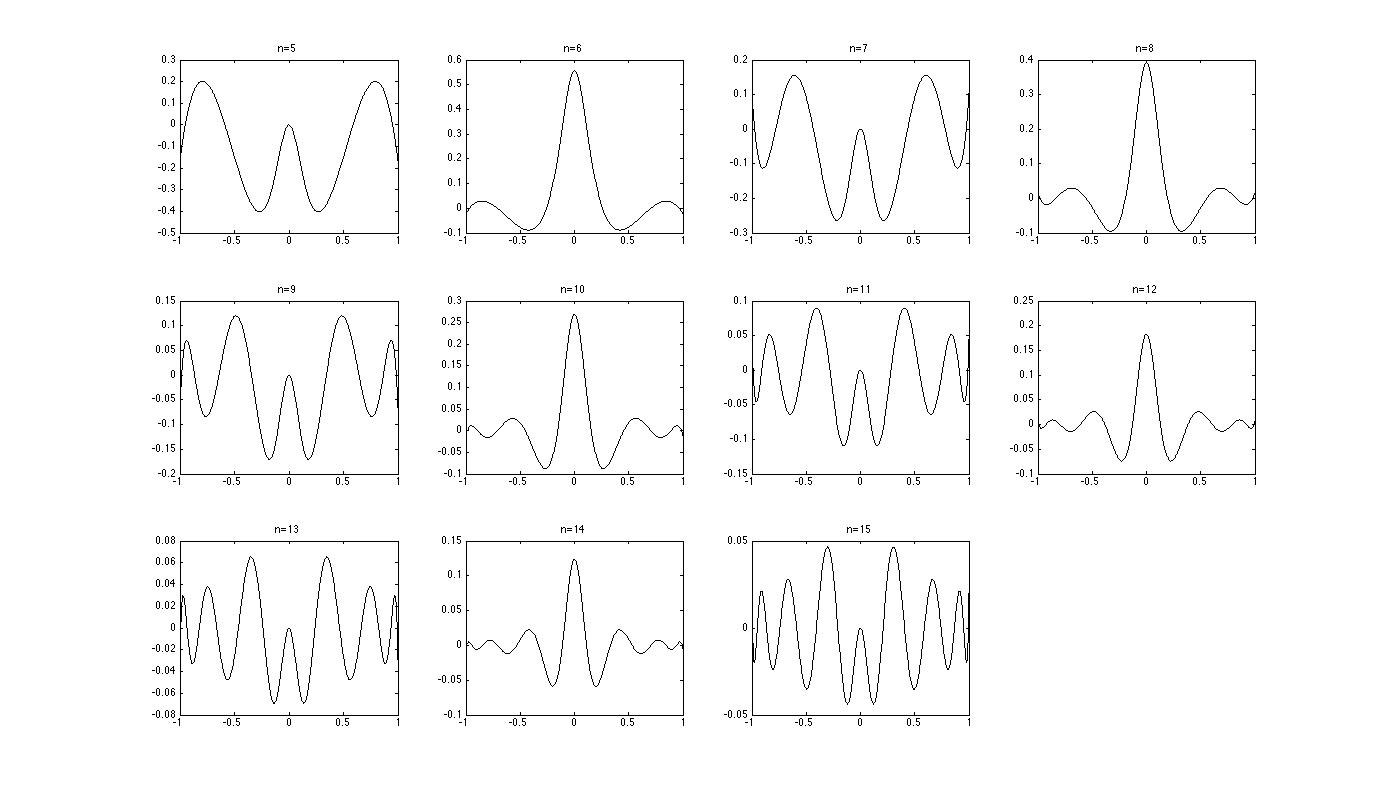
\includegraphics[width=\linewidth]{Figure/Q1_chebychev.png}
\end{figure}
\end{itemize}
\pagebreak